\section{From a surface wave to a complex envelope}
\label{sec:waves}
\subsection{Geometry, steepness, and deep water}
A linear plane wave travelling in the positive $x$ direction has elevation
\[
 \zeta(x,t)=a\cos(k_0x-\omega_0t).
\]
Its wavelength is $2\pi/k_0$, its period is $2\pi/\omega_0$, and its maximum
slope has magnitude $k_0a$. Steepness, rather than amplitude alone, measures
nonlinearity: a metre-high wave can be gentle at one wavelength and steep
at another.

\begin{assumption}[Physical setting]
The fluid is incompressible, inviscid, and irrotational, with constant
density; gravity supplies the restoring force. Surface tension, viscosity,
wind forcing, and wave breaking are excluded. The depth is treated as
infinite, the background is at rest, and $k_0a\ll1$.
\end{assumption}

At finite depth $h$, the carrier is in the deep-water regime when $k_0h\gg1$.
The infinite-depth idealization is stronger: a modulation-induced mean
response has depth scale $1/K_{\rm dim}$, often much larger than $1/k_0$.
A bottom negligible for the carrier need not be negligible for a very long
modulation. Dysthe uses an infinite lower half-space for both.

\subsection{Why use a complex variable for a real water surface?}
If $B=be^{i\beta}$, Euler's formula gives
\[
 Be^{i\theta}+B^*e^{-i\theta}=2b\cos(\theta+\beta).
\]
Magnitude and phase are stored together. A first harmonic written as
$Be^{i\theta}+\mathrm{c.c.}$ has crest amplitude $2|B|$, not $|B|$.
Here c.c. means to add the complex conjugate of the oscillatory terms;
a real mean component is included once.

A modulated surface is represented by
\begin{equation}\label{eq:surface-envelope}
 \zeta=\Zh+Be^{i\theta}+B^*e^{-i\theta}
       +\text{higher harmonics}.
\end{equation}
$B(x,y,t)$ changes little over one carrier wavelength or period. Its
magnitude controls local amplitude; its argument controls local phase.
Modulation includes changes in crest spacing and timing as well as height.

\begin{figure}[htbp]
\centering
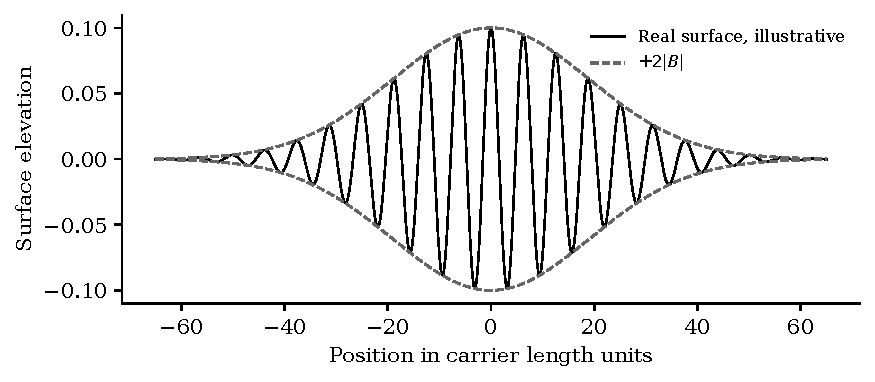
\includegraphics[width=\linewidth]{figures/carrier-envelope.pdf}
\caption{An illustrative carrier inside a slowly varying envelope at one
instant. Dashed curves are $\pm2|B|$. This is a schematic reconstruction,
not a computed Dysthe solution.}\label{fig:carrier}
\end{figure}

\subsection{Harmonics, sidebands, and the mean}
For a real narrowband wave there is a spectral cluster near $+k_0$ and a
conjugate cluster near $-k_0$. Narrowband means the width $\Delta k$ of
each cluster satisfies $\Delta k/k_0\ll1$.

A modulation creates \emph{sidebands} close to the carrier:
\[
 a[1+\delta\cos(qx)]\cos(k_0x)
 =a\cos(k_0x)+\frac{a\delta}{2}
   [\cos((k_0+q)x)+\cos((k_0-q)x)].
\]
These wavenumbers are near $k_0$ for $|q|\ll k_0$. A second
\emph{harmonic}, in contrast, has phase $2\theta$, near $2k_0$.
Nonlinear products generate harmonics even for a uniform wavetrain.
A \emph{mean} component has no fast carrier oscillation.

For $f=Be^{i\theta}+B^*e^{-i\theta}$,
\begin{equation}\label{eq:harmonic-product}
 f^2=B^2e^{2i\theta}+2|B|^2+(B^*)^2e^{-2i\theta}.
\end{equation}
A carrier-period average keeps $2|B|^2$ and removes the oscillatory terms.
A cubic product has first-harmonic coefficient $3|B|^2B$, explaining the
basic cubic structure of an envelope nonlinearity.

The average holds the slow coordinates effectively fixed. It is not an
average over the whole packet; its result can still vary in $x,y,t$.

\subsection{Potential envelope versus elevation envelope}
Dysthe writes the first-harmonic potential as
\[
 \phi=\Ph+A_{\rm dim}e^{k_0z}e^{i\theta}
 +A_{\rm dim}^*e^{k_0z}e^{-i\theta}+\cdots.
\]
The exponential describes depth decay. At leading linear order,
the dynamic surface condition gives
\begin{equation}\label{eq:AB}
 B_{\rm dim}=\frac{i\omega_0}{g}A_{\rm dim}.
\end{equation}
For a uniform carrier, $a=2|B_{\rm dim}|$. Hence the scaled potential
envelope in Dysthe (2.18) has
\[
 |A|=\frac{2k_0^2}{\omega_0}|A_{\rm dim}|=k_0a.
\]
Equal leading magnitudes do not make the envelopes interchangeable at fourth
order: their higher-order relations contain corrections.

\paperlink{Read (2.6), printed p.~107. Identify the carrier,
bound harmonics, and real mean fields.}
\checkpoint{Explain why $\mathrm{c.c.}$ makes the field real and
why the leading surface amplitude is $2|B|$.}
\clearpage
